\documentclass[12pt, a4paper,spanish]{article}
\usepackage[utf8]{inputenc}

\usepackage{lipsum} % Package to generate dummy text throughout this template
\usepackage{varwidth}
\usepackage{graphicx}

\usepackage[T1]{fontenc} % Use 8-bit encoding that has 256 glyphs
\usepackage{microtype} % Slightly tweak font spacing for aesthetics

\usepackage[hmarginratio=1:1,top=32mm,columnsep=20pt]{geometry} % Document margins
\usepackage{multicol} % Used for the two-column layout of the document
\usepackage[hang, small,labelfont=bf,up,textfont=it,up]{caption} % Custom captions under/above floats in tables or figures
\usepackage{booktabs} % Horizontal rules in tables
\usepackage{float} % Required for tables and figures in the multi-column environment - they need to be placed in specific locations with the [H] (e.g. \begin{table}[H])
\usepackage{hyperref} % For hyperlinks in the PDF

\usepackage{lettrine} % The lettrine is the first enlarged letter at the beginning of the text
\usepackage{paralist} % Used for the compactitem environment which makes bullet points with less space between them

\usepackage{abstract} % Allows abstract customization
\renewcommand{\abstractnamefont}{\normalfont\bfseries} % Set the "Abstract" text to bold
\renewcommand{\abstracttextfont}{\normalfont\small\itshape} % Set the abstract itself to small italic text

\usepackage{titlesec} % Allows customization of titles
\renewcommand\thesection{\Roman{section}} % Roman numerals for the sections
\renewcommand\thesubsection{\Roman{subsection}} % Roman numerals for subsections
\titleformat{\section}[block]{\large\scshape\centering}{\thesection.}{1em}{} % Change the look of the section titles
\titleformat{\subsection}[block]{\large}{\thesubsection.}{1em}{} % Change the look of the section titles

\usepackage{fancyhdr} % Headers and footers
\pagestyle{fancy} % All pages have headers and footers
\fancyhead{} % Blank out the default header
\fancyfoot{} % Blank out the default footer
\fancyhead[C]{Sergio García Prado $\bullet$ Febrero 2016 $\bullet$ Investigación de Operaciones} % Custom header text
\fancyfoot[RO,LE]{\thepage} % Custom footer text

%----------------------------------------------------------------------------------------
%	TITLE SECTION
%----------------------------------------------------------------------------------------

\title{\vspace{-15mm}\fontsize{24pt}{10pt}\selectfont\textbf{Investigación de Operaciones}} % Article title

\author{
\large
\textsc{Sergio García Prado}\\[2mm] % Your name
\normalsize Universidad de Valladolid \\ % Your institution
\vspace{-5mm}
}
\date{}

%----------------------------------------------------------------------------------------

\begin{document}

	\maketitle % Insert title

	\thispagestyle{fancy} % All pages have headers and footers

%----------------------------------------------------------------------------------------
%	ABSTRACT
%----------------------------------------------------------------------------------------

	\begin{abstract}
		\noindent Investigación de Operaciones
	\end{abstract}

	\section{Orígenes}

		\paragraph{}
		Cuando comenzó la Segunda Guerra Mundial, había un pequeño grupo de investigadores militares, encabezados por A. P. Rowe, interesados en el uso militar de una técnica conocida como radioubicación (o radiolocalización), que desarrollaron científicos civiles. Algunos historiadores consideran que esta investigación es el punto inicial de la investigación de operaciones. Otros creen que los estudios que tienen las características del trabajo de investigación de operaciones aparecieron posteriormente. Algunos consideran que su comienzo está en el análisis y solución del bloqueo naval de Siracusa que Arquímedes presentó al tirano de esa ciudad, en el siglo III A.C. F. W. Lanchester, en Inglaterra, justo antes de la primera guerra mundial, desarrolló relaciones matemáticas sobre la potencia balística de las fuerzas opositoras que, si se resolvían tomando en cuenta el tiempo, podían determinar el resultado de un encuentro militar. Thomas Alva Edison también realizó estudios de guerra antisubmarina. Ni los estudios de Lanchester ni los de Edison tuvieron un impacto inmediato; junto con los de Arquímedes, constituyen viejos ejemplos del empleo de científicos para determinar la decisión óptima en las guerras, optimizando los ataques. \cite{wikipedia_IO}

		\paragraph{}
		En agosto de 1940 se organizó un grupo de 20 investigadores, bajo la dirección de P. M. S. Blackett, de la Universidad de Mánchester, para estudiar el uso de un nuevo sistema antiaéreo controlado por radar. Se conoció al grupo de investigación como “el Circo de Blackett”, nombre que no parece desatinado a la luz de sus antecedentes y orígenes diversos. El grupo estaba formado por tres fisiólogos, dos fisicomatemáticos, un astrofísico, un oficial del ejército, un topógrafo, un físico general y dos matemáticos. Generalmente se acepta que la formación de este grupo constituye el inicio de la investigación de operaciones. \cite{wikipedia_IO}

		\paragraph{}
		Al terminar la guerra, el éxito de la IO en las actividades bélicas generó gran interés debido a las posibilidades de aplicarla en un ámbito distinto al militar. Una vez que la explosión industrial posterior a la guerra siguió su curso, los problemas provocados por el aumento de la complejidad y la especialización de las organizaciones pasaron de nuevo al primer plano. Entonces comenzó a ser evidente para un gran número de personas, entre ellas los consultores industriales que habían trabajado con o para los equipos de IO durante la guerra, que estos problemas eran en esencia los mismos que los que debían enfrentar los militares pero en un contexto diferente. Al inicio de la década de los años cincuenta, estos visionarios introdujeron el uso de la investigación de operaciones en una serie de organizaciones industriales, de negocios y del gobierno. Desde entonces, se ha desarrollado con rapidez. \cite{hillier_lieberman_IO}

		\paragraph{}
		Un factor que dio gran impulso al desarrollo de este campo fue la revolución de las computadoras. El manejo eficaz de los complejos problemas inherentes a la IO casi siempre requiere un gran número de cálculos. Realizarlos de forma manual puede resultar casi imposible, por lo cual el desarrollo de la computadora electrónica digital, con su capacidad para hacer cálculos aritméticos, miles o tal vez millones de veces más rápido que los seres humanos, fue una gran ayuda para esta disciplina.	\cite{hillier_lieberman_IO}

		\begin{figure}[H]
				\centering
				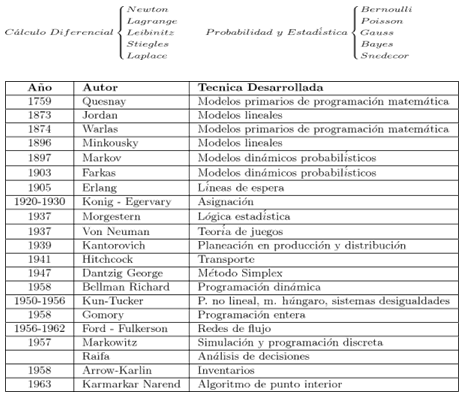
\includegraphics[width=120mm]{res/desarrollo-historico-de-la-investigacion-de-operaciones.png}
				\caption{Evolución histórica de la Investigación Operativa \protect\cite{gestiopolis_IO_history}}
			\end{figure}


	\section{Naturaleza}
		\paragraph{}
		La investigación operativa es una moderna disciplina científica que se caracteriza por la aplicación de teoría, métodos y técnicas especiales, para buscar la solución de problemas de administración, organización y control que se producen en los diversos sistemas que existen en la naturaleza y los creados por el ser humano, tales como las organizaciones a las que identifica como sistemas organizados, sistemas físicos, económicos, ecológicos, educacionales, de servicio social, etcétera.\cite{wikipedia_IO}

		\paragraph{}
		El objetivo más importante de la aplicación de la investigación operativa es apoyar en la toma óptima de decisiones en los sistemas y en la planificación de sus actividades. El enfoque fundamental de la investigación operativa es el enfoque de sistemas, por el cual, a diferencia del enfoque tradicional, se estudia el comportamiento de todo un conjunto de partes o sub-sistemas que interaccionan entre sí, se identifica el problema y se analizan sus repercusiones, y se buscan soluciones integrales que beneficien al sistema como un todo. Para hallar la solución, la investigación operativa generalmente representa el problema como un modelo matemático, que se analiza y evalúa previamente.\cite{wikipedia_IO}

		\paragraph{}
		En relación a lo anterior se necesita gente capacitada, en el ámbito de las matemáticas, estadísticas y teoría de probabilidades, al igual que en economía, administración de empresas, ciencias de la computación, ingeniería, ciencias físicas, ciencias de comportamiento y, por supuesto, en las técnicas especiales de investigación de operaciones. La mezcla de todas estas habilidades ayuda a desarrollar la mejor toma de decisiones, ejerciéndolas en los métodos de investigación de operaciones.\cite{gestiopolis_IO}



	\section{Influencia}
		\paragraph{}
		Investigación de Operaciones

	\section{Etapas del estudio}
		\paragraph{}

		\subsection{Formulación y definición del problema}

			\paragraph{}
			Descripción de los objetivos del sistema, es decir, qué se desea optimizar; identificar las variables implicadas, ya sean controlables o no; determinar las restricciones del sistema. También hay que tener en cuenta las alternativas posibles de decisión y las restricciones para producir una solución adecuada.\cite{invdeop_IO}

		\subsection{Construcción del modelo}

			\paragraph{}
			El investigador de operaciones debe decidir el modelo a utilizar para representar el sistema. Debe ser un modelo tal que relacione a las variables de decisión con los parámetros y restricciones del sistema. Los parámetros (o cantidades conocidas) se pueden obtener ya sea a partir de datos pasados o ser estimados por medio de algún método estadístico. Es recomendable determinar si el modelo es probabilístico o determinístico. El modelo puede ser matemático, de simulación o heurístico, dependiendo de la complejidad de los cálculos matemáticos que se requieran.\cite{invdeop_IO}

		\subsection{Solución del modelo}

			\paragraph{}
			Una vez que se tiene el modelo, se procede a derivar una solución matemática empleando las diversas técnicas y métodos matemáticos para resolver problemas y ecuaciones. Debemos tener en cuenta que las soluciones que se obtienen en este punto del proceso, son matemáticas y debemos interpretarlas en el mundo real. Además, para la solución del modelo, se deben realizar análisis de sensibilidad, es decir, ver como se comporta el modelo a cambios en las especificaciones y parámetros del sistema. Esto se hace, debido a que los parámetros no necesariamente son precisos y las restricciones pueden estar equivocadas.\cite{invdeop_IO}

		\subsection{Validación del modelo}

			\paragraph{}
			La validación de un modelo requiere que se determine si dicho modelo puede predecir con certeza el comportamiento del sistema. Un método común para probar la validez del modelo, es someterlo a datos pasados disponibles del sistema actual y observar si reproduce las situaciones pasadas del sistema. Pero como no hay seguridad de que el comportamiento futuro del sistema continúe replicando el comportamiento pasado, entonces siempre debemos estar atentos de cambios posibles del sistema con el tiempo, para poder ajustar adecuadamente el modelo.\cite{invdeop_IO}

		\subsection{Implementación de resultados}

			\paragraph{}
			Consiste en traducir los resultados del modelo validado en instrucciones para el usuario o los ejecutivos responsables que serán tomadores de decisiones.\cite{invdeop_IO}


%----------------------------------------------------------------------------------------
%	Bibliographic references
%----------------------------------------------------------------------------------------
	\begin{thebibliography}{9}

		\bibitem{wikipedia_IO}
		Wikipedia. Investigación de Operaciones. \url{https://es.wikipedia.org/wiki/Investigación_de_operaciones}

		\bibitem{hillier_lieberman_IO}
		Hillier / Lieberman. Introducción a la Investigacion de Operaciones.

		\bibitem{gestiopolis_IO_history}
		Gestiopolis. Desarrollo histórico de la investigación de operaciones. \url{http://www.gestiopolis.com/desarrollo-historico-de-la-investigacion-de-operaciones/}

		\bibitem{gestiopolis_IO}
		Gestiopolis. Investigación de operaciones, qué es, historia y metodología. \url{http://www.gestiopolis.com/investigacion-de-operaciones-que-es-historia-y-metodologia/}

		\bibitem{invdeop_IO}
		InvdeOp. Fases de la Investigación de Operaciones. \url{https://invdeop.wordpress.com/2011/04/07/fases-de-la-investigacion-de-operaciones/}

	\end{thebibliography}

\end{document}
